\section{Convergence Power Spectrum}
The matter power spectrum, \( P(k) \), is a fundamental quantity in cosmology that characterizes the distribution of dark matter density fluctuations in Fourier space. It is defined as the Fourier transform of the two-point correlation function of the dark matter density field, \( \delta(\mathbf{x}) \) \citep{2001PhR...340..291B}. Mathematically, the matter power spectrum is expressed as:
\begin{equation}
    \langle \tilde{\delta}(\mathbf{k}) \tilde{\delta}(\mathbf{k}') \rangle = (2\pi)^3 \delta^{(3)}(\mathbf{k} + \mathbf{k}') P(k),
    \label{eq:matter_power_spectrum}
\end{equation}
where \( \tilde{\delta}(\mathbf{k}) \) represents the Fourier transform of the density contrast \( \delta(\mathbf{x}) \), and \( \delta^{(3)} \) is the three-dimensional Dirac delta function ensuring statistical isotropy and homogeneity.

In the context of weak gravitational lensing, the matter power spectrum \( P(k) \) is not directly observable. Instead, observations yield the angular power spectrum of the convergence field, \( C_{\ell}^{\kappa\kappa} \), which encapsulates the statistical properties of the convergence \( \kappa(\boldsymbol{\theta}) \) across the sky \citep{2001PhR...340..291B}. The convergence power spectrum, \( P_{\kappa}(\ell) \), is defined through the relation:
\begin{equation}
    \langle \tilde{\kappa}(\boldsymbol{\ell}) \tilde{\kappa}(\boldsymbol{\ell}') \rangle = (2\pi)^2 \delta^{(2)}(\boldsymbol{\ell} + \boldsymbol{\ell}') P_{\kappa}(\ell),
    \label{eq:convergence_power_spectrum}
\end{equation}
where \( \tilde{\kappa}(\boldsymbol{\ell}) \) is the Fourier transform of the convergence field \( \kappa(\boldsymbol{\theta}) \), and \( \delta^{(2)} \) is the two-dimensional Dirac delta function.

The convergence field \( \kappa(\boldsymbol{\theta}) \) can be expressed as a weighted projection of the matter density contrast along the line of sight (see Eq.~\eqref{eq:convergence_integral}):
\begin{equation}
    \kappa(\boldsymbol{\theta}) = \int_0^{\chi_s} d\chi \, W(\chi) \, \delta_m\left(\chi \boldsymbol{\theta}, \chi\right),
    \label{eq:kappa_projection}
\end{equation}
where \( W(\chi) \) is the lensing kernel, \( \chi \) is the comoving radial distance.

Recognizing the Fourier transform of the matter density field \( \delta_m\left(\chi \boldsymbol{\theta}, \chi\right) \), we write:
\begin{equation}
    \delta_m\left(\chi \boldsymbol{\theta}, \chi\right) = \int \frac{d^3\mathbf{k}}{(2\pi)^3} \tilde{\delta}(\mathbf{k}) e^{i \mathbf{k} \cdot \mathbf{x}},
    \label{eq:delta_m_fourier}
\end{equation}
where \( \mathbf{x} = (\chi \boldsymbol{\theta}, \chi) \) is the comoving position vector. Substituting this into the Fourier transform of the convergence field \( \tilde{\kappa}(\boldsymbol{\ell}) \), we obtain:
\begin{eqnarray}
    \tilde{\kappa}(\boldsymbol{\ell}) &=& \int_0^{\chi_s} d\chi \, W(\chi) \int d\boldsymbol{\theta} \, e^{-i \boldsymbol{\ell} \cdot \boldsymbol{\theta}} \delta_m\left(\chi \boldsymbol{\theta}, \chi\right) \nonumber \\
    &=& \int_0^{\chi_s} d\chi \, W(\chi) \int \frac{d^3\mathbf{k}}{(2\pi)^3} \tilde{\delta}(\mathbf{k}) e^{i k_\parallel \chi} \int d\boldsymbol{\theta} \, e^{-i \boldsymbol{\ell} \cdot \boldsymbol{\theta}} e^{i \chi \mathbf{k}_\perp \cdot \boldsymbol{\theta}} \nonumber \\
    &=& \int_0^{\chi_s} d\chi \, W(\chi) \int \frac{dk_\parallel}{2\pi} \frac{d^2\mathbf{k}_\perp}{(2\pi)^2} \tilde{\delta}_m(k_\parallel, \mathbf{k}_\perp) e^{i k_\parallel \chi} \int d\boldsymbol{\theta} \, e^{-i (\boldsymbol{\ell} - \chi \mathbf{k}_\perp) \cdot \boldsymbol{\theta}} \nonumber \\
    &=& \int_0^{\chi_s} d\chi \, \frac{W(\chi)}{\chi^2} \int \frac{dk_\parallel}{2\pi} \tilde{\delta}_m\left(k_\parallel, \frac{\boldsymbol{\ell}}{\chi}\right) e^{i k_\parallel \chi},
    \label{eq:kappa_fourier_final}
\end{eqnarray}
where \( \mathbf{k}_\perp \) and \( k_\parallel \) are the components of \( \mathbf{k} \) perpendicular and parallel to the line of sight, respectively.

Next, we compute the ensemble average of the Fourier transform of the convergence field:
\begin{eqnarray}
    \langle \tilde{\kappa}(\boldsymbol{\ell}) \tilde{\kappa}(\boldsymbol{\ell}') \rangle 
    &=& \int_0^{\chi_s} d\chi \, \frac{W(\chi)}{\chi^2} \int_0^{\chi_s} d\chi' \, \frac{W(\chi')}{\chi'^2} 
        \int \frac{dk_\parallel}{2\pi} \int \frac{dk'_\parallel}{2\pi} \nonumber \\
    && \times \langle \tilde{\delta}_m\left(k_\parallel, \frac{\boldsymbol{\ell}}{\chi}\right) 
       \tilde{\delta}_m\left(k'_\parallel, \frac{\boldsymbol{\ell}'}{\chi'}\right) \rangle 
       e^{i k_\parallel \chi} e^{i k'_\parallel \chi'} \nonumber \\
    [2ex]
    &=& \int_0^{\chi_s} d\chi \, \frac{W(\chi)}{\chi^2} \int_0^{\chi_s} d\chi' \, \frac{W(\chi')}{\chi'^2} 
        \int \frac{dk_\parallel}{2\pi} e^{i k_\parallel (\chi - \chi')} \nonumber \\
    && \times (2\pi)^2 \delta^{(2)}\left(\frac{\boldsymbol{\ell}}{\chi} + \frac{\boldsymbol{\ell}'}{\chi'}\right) 
       P_m\left(\sqrt{k_\parallel^2 + \frac{\ell^2}{\chi^2}}\right) \nonumber 
    \label{eq:kappa_power_spectrum}
\end{eqnarray}
where in the last step we have applied the Limber approximation \citep{1954ApJ...119..655L}, which assumes \( k_\parallel \ll \ell/\chi \).
Under the Limber approximation, the integral simplifies as:
\begin{equation}
    \int \frac{dk_\parallel}{2\pi} e^{i k_\parallel (\chi - \chi')} P_m\left(\sqrt{k_\parallel^2 + \frac{\ell^2}{\chi^2}}\right) \approx P_m\left(\frac{\ell}{\chi}\right) \delta(\chi - \chi'),
    \label{eq:limber_approximation}
\end{equation}
where \( P_m(k) \) is evaluated at \( k = \ell/\chi \).
Substituting this into Eq.~\eqref{eq:kappa_power_spectrum}, we obtain:
\begin{equation}
    \langle \tilde{\kappa}(\boldsymbol{\ell}) \tilde{\kappa}(\boldsymbol{\ell}') \rangle = (2\pi)^2 \delta^{(2)}(\boldsymbol{\ell} + \boldsymbol{\ell}') \int_0^{\chi_s} d\chi \, \frac{W^2(\chi)}{\chi^2} P_m\left(\frac{\ell}{\chi}; \chi\right),
    \label{eq:kappa_power_spectrum_final}
\end{equation}
where \( P_m\left(\frac{\ell}{\chi}; \chi\right) \) denotes the matter power spectrum evaluated at wavenumber \( k = \ell/\chi \) and at the comoving distance \( \chi \).
Finally, equating this result with the definition of the convergence power spectrum in Eq.~\eqref{eq:convergence_power_spectrum}, we derive the expression for \( C_{\ell}^{\kappa\kappa} \):
\begin{equation}
    C_{\ell}^{\kappa\kappa} = \int_0^{\chi_s} d\chi \, \frac{W^2(\chi)}{\chi^2} P_m\left(\frac{\ell}{\chi}; \chi\right).
    \label{eq:convergence_power_spectrum_final}
\end{equation}
This relation demonstrates how the observable convergence power spectrum \( C_{\ell}^{\kappa\kappa} \) is sourced by the underlying matter power spectrum \( P_m(k; \chi) \) integrated along the line of sight.

\subsection{\texttt{Halofit} Model}
Based on the halo models (discussed in Sec.~\ref{sec:halo}), Halofit model is a widely used prescription to compute the non-linear matter power spectrum \( P(k) \) from the linear power spectrum \( P_{\mathrm{L}}(k) \) \citep{2003MNRAS.341.1311S, 2012ApJ...761..152T}. In the Halofit regime, the power spectrum is consists of two terms:
\begin{equation}
    P(k) = P_{\mathrm{1h}}(k) + P_{\mathrm{2h}}(k),
    \label{eq:halofit_model}
\end{equation}
where the two-halo term \( P_{\mathrm{2h}}(k) \) captures the contribution from large-scale linear structures, given by:   
\begin{equation}
    P_{\mathrm{2h}}(k) = P_{\mathrm{L}}(k) \left[ \frac{1}{\bar{\rho}} \int dM \, b(M) n(M) \tilde{\rho}(k, M) \right]^2,
    \label{eq:halofit_1h}
\end{equation}
and one-halo term $P_{\mathrm{1h}}(k)$ accounts for the contribution from small-scale non-linear structures, defined as:
\begin{equation}
    P_{\mathrm{1h}}(k) = \frac{1}{\bar{\rho}^2 (2\pi)^3} \int dM \, n(M) \left| \tilde{\rho}(k, M) \right|^2.
    \label{eq:halofit_2h}
\end{equation}
Here, \( \bar{\rho} \) is the mean matter density, \( n(M) dM \) is the halo mass function, \( b(M) \) is the halo bias, and \( \tilde{\rho}(k, M) \) is the Fourier transform of the halo density profile. 
Those two terms are then approximated into empirical fitting formulae and calibrated against \( N \)-body simulations.

The one-halo term resembles a shot noise spectrum on large scales but is progressively reduced on small scales due to the filtering effects of halo profiles and the mass function. Conversely, the two-halo term modifies the relative correlations of halos beyond what is predicted by linear theory and becomes negligible on small scales. 

\section{Convergence Bispectrum}
The bispectrum, \( B(k) \), serves as the Fourier counterpart to the three-point correlation function and is the lowest-order statistical quantity capable of characterizing non-Gaussianity in the matter distribution \citep{2002PhR...367....1B}. While the power spectrum effectively captures Gaussian fluctuations through two-point statistics, the bispectrum provides deeper insights by incorporating three-point correlations, thereby unveiling more complex structures in the cosmic density field \citep{1999ApJ...517..531S, 2004MNRAS.348..897T}.

Analogous to the angular power spectrum, the convergence bispectrum can be expressed as the ensemble average of three Fourier-transformed convergence modes, \( \tilde{\kappa} \) \citep{2005PhRvD..72h3001D}:
\begin{equation}
    \langle \tilde{\kappa}(\mathbf{\ell}_1) \tilde{\kappa}(\mathbf{\ell}_2) \tilde{\kappa}(\mathbf{\ell}_3) \rangle = (2\pi)^2 \delta_{D}(\mathbf{\ell}_1 + \mathbf{\ell}_2 + \mathbf{\ell}_3) B^\kappa_{\ell_1 \ell_2 \ell_3},
    \label{eq:convergence_bispectrum_def}
\end{equation}
Building upon the derivations analogous to Equations~\eqref{eq:kappa_fourier_final} through~\eqref{eq:kappa_power_spectrum_final}, the convergence bispectrum can be expressed as:
\begin{equation}
    B_{\ell_1 \ell_2 \ell_3}^\kappa = \int_0^{\chi_s} d\chi \, \frac{W^3(\chi)}{\chi^4} B_m\left( \frac{\ell_1}{\chi}, \frac{\ell_2}{\chi}, \frac{\ell_3}{\chi}; \chi \right),
    \label{eq:convergence_bispectrum}
\end{equation}
where \( B_m(k_1, k_2, k_3, z) \) denotes the matter bispectrum at redshift \( z \), and \( W(\chi) \) is the lensing kernel. 

The bispectrum depends not only on the magnitudes of the wavevectors but also on the shapes formed by the triplet \( (\boldsymbol{k}_1, \boldsymbol{k}_2, \boldsymbol{k}_3) \), constrained by the condition \( \boldsymbol{k}_1 + \boldsymbol{k}_2 + \boldsymbol{k}_3 = 0 \). Different triangle configurations (e.g.\, equilateral, squeezed, isoceles) probe different physical processes and scales in the Universe \citep{2005PhRvD..72h3001D}.

\subsection{\texttt{BiHalofit} Model}
The \texttt{BiHalofit} model \citep{2020ApJ...895..113T} extends the Halofit prescription to compute the non-linear matter bispectrum \( B_m(k_1, k_2, k_3) \) from the linear matter power spectrum \( P_{\mathrm{L}}(k) \). The bispectrum is decomposed into one-halo and three-halo terms, given by:
\begin{equation}
    B_m(k_1, k_2, k_3) = B_{\mathrm{1h}}(k_1, k_2, k_3) + B_{\mathrm{3h}}(k_1, k_2, k_3),
    \label{eq:bihalofit_model}
\end{equation}
The one-halo term describes the correlation in an individual halo, and the three-halo term captures the correlation between three different halos. Because the two-halo term is subdominant in most of the triangle configurations (except at the squeezed limit; \citealt{2011A&A...532A...4V}), it is neglected in the \texttt{BiHalofit} model.

The one-halo term is given by:
\begin{equation}
    B_{1h}\left(k_1, k_2, k_3\right)=\int d M \frac{d n(M)}{d M}\left(\frac{M}{\bar{\rho}}\right)^3 u\left(k_1 ; M\right) u\left(k_2 ; M\right) u\left(k_3 ; M\right)
    \label{eq:bihalofit_1h}
\end{equation}
where \( u(k; M) \) is the Fourier transform of the scaled halo density profile $\rho(r; M)/M$. The three-halo term is given by:
\begin{equation}
    B_{3h}\left(k_1, k_2, k_3\right)=2\left[F_2\left(\boldsymbol{k}_1, \boldsymbol{k}_2\right)+\frac{I_1^2\left(k_3\right)}{2 I_1^1\left(k_3\right)}\right] I_1^1\left(k_1\right) I_1^1\left(k_2\right) I_1^1\left(k_3\right) P_{\mathrm{L}}\left(k_1\right) P_{\mathrm{L}}\left(k_2\right)+2 \text { perm. }
    \label{eq:bihalofit_3h}
\end{equation}
with 
\begin{equation}
    I_1^\beta(k)=\int d M \frac{d n(M)}{d M} \frac{M}{\bar{\rho}} b_\beta(M) u(k ; M)
    \label{eq:bihalofit_3h_integral}
\end{equation}
and
\begin{equation}
    F_2\left(\boldsymbol{k}_1, \boldsymbol{k}_2\right)=\frac{5}{7}+\frac{1}{2}\left(\frac{k_1}{k_2}+\frac{k_2}{k_1}\right) \mu_{12}+\frac{2}{7} \mu_{12}^2
    \label{eq:bihalofit_3h_F2}
\end{equation}
which is given at the tree level (leading order) in perturbation theory \citep{2002PhR...367....1B}.


\section{Probability Density Functions} \label{sec:pdfs}
The Probability Density Function (PDF) of the convergence field, $\kappa$, provides a fundamental statistical characterization of the field's one-point distribution. By encompassing all moments and cumulants, the PDF captures both Gaussian and non-Gaussian features intrinsic to the convergence field.

To effectively suppress noise and small-scale fluctuations, the convergence map $\kappa(\hat{\mathbf{n}})$ is first smoothed with a Gaussian kernel. The smoothed convergence field, $\kappa_{\mathrm{smooth}}(\hat{\mathbf{n}})$, is defined as:
\begin{equation}
    \kappa_{\mathrm{smooth}}(\hat{\mathbf{n}}) = \int_{S^2} \kappa(\hat{\mathbf{n}}') W(\hat{\mathbf{n}} - \hat{\mathbf{n}}') \, d\hat{\mathbf{n}}',
    \label{eq:smoothing}
\end{equation}
where $W(\theta)$ is the Gaussian smoothing kernel given by:
\begin{equation}
    W(\theta) = \frac{1}{2\pi \sigma_{\theta}^2} \exp\left( -\frac{\theta^2}{2 \sigma_{\theta}^2} \right),
    \label{eq:gaussian_kernel}
\end{equation}
with $\theta = \arccos(\hat{\mathbf{n}} \cdot \hat{\mathbf{n}}')$ representing the angular separation between the points $\hat{\mathbf{n}}$ and $\hat{\mathbf{n}}'$ on the unit sphere $S^2$, and $\sigma_{\theta}$ is the smoothing scale. To standardize the statistical analysis, the smoothed convergence values are normalized by their standard deviation. The normalized smoothed convergence, $\tilde{\kappa}_{\mathrm{smooth}, i}$, is defined as:
\begin{equation}
    \nu_{i} = \frac{\kappa_{\mathrm{smooth}, i} - \langle \kappa_{\mathrm{smooth}} \rangle}{\sigma_{\mathrm{smooth}}},
    \label{eq:kappa_smooth_normalized}
\end{equation}
where:
\begin{equation}
    \langle \kappa_{\mathrm{smooth}} \rangle = \frac{1}{N_{\mathrm{pix}}} \sum_{i=1}^{N_{\mathrm{pix}}} \kappa_{\mathrm{smooth}, i}, \quad \sigma_{\mathrm{smooth}}^2 = \sigma_{\mathrm{signal}}^2 + \sigma_{\mathrm{noise}}^2.
    \label{eq:normalization}
\end{equation}
Formally, the PDF \( P(\nu) \) is defined such that:
\begin{equation}
    P(\nu) \, d\nu = \mathrm{Prob}(\nu \leq \nu' \leq \nu + d\nu),
\end{equation}
where \(\mathrm{Prob}\) denotes the probability that the normalized convergence \(\nu'\) lies within the interval \([\nu, \nu + d\nu]\).

For a discrete set of normalized convergence measurements \(\{\nu_i\}_{i=1}^{N_{\mathrm{pix}}}\) obtained from \(N_{\mathrm{pix}}\) pixels, the PDF can be represented using the Dirac delta function \(\delta_D\):
\begin{equation}
    P(\nu) = \frac{1}{N_{\mathrm{pix}}} \sum_{i=1}^{N_{\mathrm{pix}}} \delta_D(\nu - \nu_i).
    \label{eq:pdf_delta}
\end{equation}
This expression effectively constructs the PDF by summing over all pixel values, assigning a weight to each normalized convergence measurement \(\nu_i\) at its exact value.

In practical applications, however, the Dirac delta function is not computationally feasible. Instead, we approximate the PDF by discretizing the normalized convergence values into bins of finite width \(\Delta\nu\). This leads to a binned estimator:
\begin{equation}
    P(\nu) \approx \frac{1}{N_{\mathrm{pix}} \Delta\nu} \sum_{i=1}^{N_{\mathrm{pix}}} \Theta\left(\left|\nu_i - \nu\right| \leq \frac{\Delta\nu}{2}\right),
    \label{eq:pdf_binned}
\end{equation}
where \(\Theta(x)\) is the Heaviside step function. This estimator counts the number of normalized convergence \(\nu_i\) that fall within each bin centered at \(\nu\), normalizing by the total number of pixels and the bin width \(\Delta\nu\).

\subsection{\texttt{hmpdf} Model}
The \texttt{hmpdf} model \citep{2020PhRvD.102l3545T} presents a halo-model formalism to compute the weak lensing convergence PDF, and its covariance matirix. The one-point $P(\kappa_a)$ and two-point $P(\kappa_a, \kappa_b; \phi)$ PDFs are separated into one-halo and two-halo terms as:
\begin{equation}
    P_{\text{1pt/2pt}} = P^{1h}_{\text{1pt/2pt}}P^{2h}_{\text{1pt/2pt}},
    \label{eq:hmpdf}
\end{equation}
for exact formulae, see \cite{2020PhRvD.102l3545T}. Expanding the exponentials to the first order, the $p$-th order of the one-halo term describes overlaps of $p$ halos along the line of sight. The two-halo term arises from the dependence of halo density on the underlying matter density field.

\section{Peak and Minimum Counts}
\label{sec:peak_min_counts}
Local maxima (peaks) and minima in convergence field correspond to regions of over-densities and under-densities, respectively. Analyzing the statistics of these extrema offers insights into the non-Gaussian features of the matter distribution, providing a powerful tool to constrain cosmological models beyond traditional two-point statistics like the power spectrum \citep{2000ApJ...530L...1J, 2010MNRAS.402.1049D}.

The $i$-th pixel in the normalized convergence map, $\nu$ is identified as a peak or a minimum by comparing its value with those of its neighboring pixels. Formally, let $\mathcal{N}(i)$ denote the set of neighboring pixels adjacent to pixel $i$. The conditions for a pixel to be classified as a peak or a minimum are then defined as:
\begin{align}
    \text{Peak Condition:} \quad & \kappa_{\mathrm{smooth}, i} > \kappa_{\mathrm{smooth}, j} \quad \forall \, j \in \mathcal{N}(i), \label{eq:peak_condition} \\
    \text{Minimum Condition:} \quad & \kappa_{\mathrm{smooth}, i} < \kappa_{\mathrm{smooth}, j} \quad \forall \, j \in \mathcal{N}(i). \label{eq:min_condition}
\end{align}
These conditions ensure that peaks are local maxima and minima are local minima in the convergence field. Figure~\ref{fig:peak_min} illustrates the identification of peaks (red circles) and minima (blue circles) in the smoothed convergence map $\kappa_{\mathrm{smooth}}(\hat{\mathbf{n}})$.
\begin{figure}[ht]
    \centering
    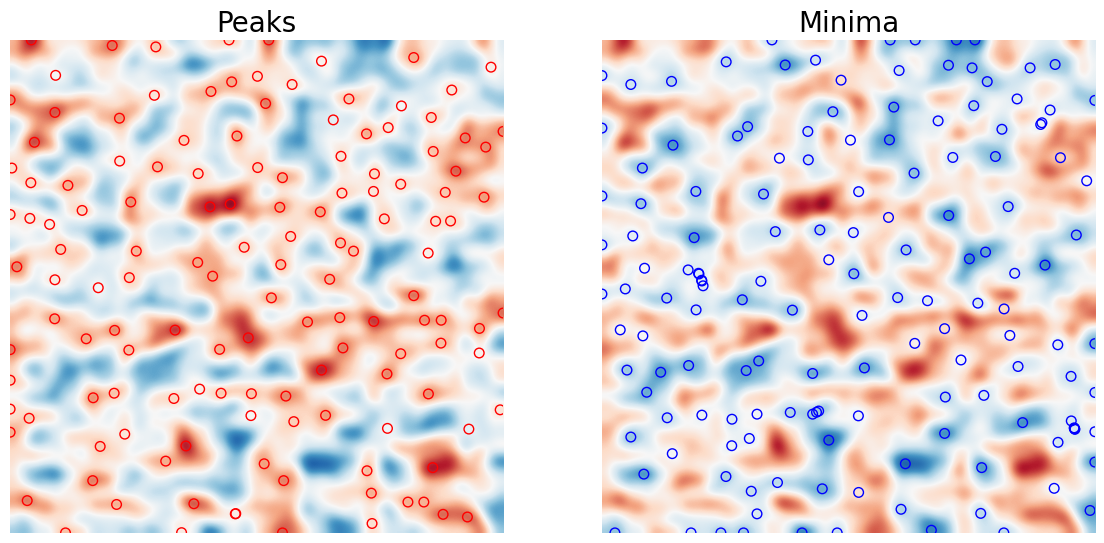
\includegraphics[width=0.8\textwidth]{figures/peaks_minima.png}
    \caption{Identification of peaks and minima in a smoothed convergence map. The left panel shows the smoothed convergence field $\kappa_{\mathrm{smooth}}(\hat{\mathbf{n}})$ with peaks (red circles) satisfying the peak condition (Equation~\eqref{eq:peak_condition}), and the right panel highlights the minima (blue circles) satisfying the minimum condition (Equation~\eqref{eq:min_condition}).}
    \label{fig:peak_min}
\end{figure}

The noise properties of peaks can be analytically described using Gaussian statistics \citep{1986ApJ...304...15B, 1987MNRAS.226..655B}. Due to the symmetry of a Gaussian field, the expected number density of minima below $-\nu$ is equal to that of peaks above $\nu$, $N_{\mathrm{\min}}(-\nu) = N_{\mathrm{peak}}(\nu)$.

Different approaches to analytically predict weak lensing peak counts have been developed over the recent years. One milestone is the model for Gaussian random Field developed by \citet{1986ApJ...304...15B}, and the extention to the weak lensing field by \citet{2010A&A...519A..23M}. Another popular way to analyze weak lensing data is to compare the measured peak counts to weak lensing maps generated by N-body simulations \citep{2016MNRAS.463.3653K, 2018MNRAS.474..712M, 2021JCAP...01..028Z}.

\section{Minkowski Functionals}
\label{sec:minkowski_functionals}
Minkowski functionals are powerful morphological descriptors derived from integral geometry, widely used to quantify the geometry and topology of spatial structures \citep{2024arXiv241000401A}. 

For a two-dimensional normalized convergence field $\nu(\hat{\mathbf{n}})$ with zero mean and variance $\sigma_0^2$, the excursion set $\Sigma(\nu_0)$ at threshold $\nu_0$ is defined as the set of points where the field exceeds a certain threshold value:
\begin{equation}
    \Sigma(\nu_0) = \left\{ \hat{\mathbf{n}} \in S^2 \ \bigg| \ \nu(\hat{\mathbf{n}}) > \nu_0 \right\}.
\end{equation}
Figure~\ref{fig:excursion_sets} shows $\Sigma(\nu_0)$ for increasing threshold values $\nu_0 = 0.5, 1, 1.5$ and $2$. As the threshold increases, the size and connectivity of the excursion sets diminish, reflecting the decreasing number of high-value regions in the field.
\begin{figure}[ht]
    \centering
    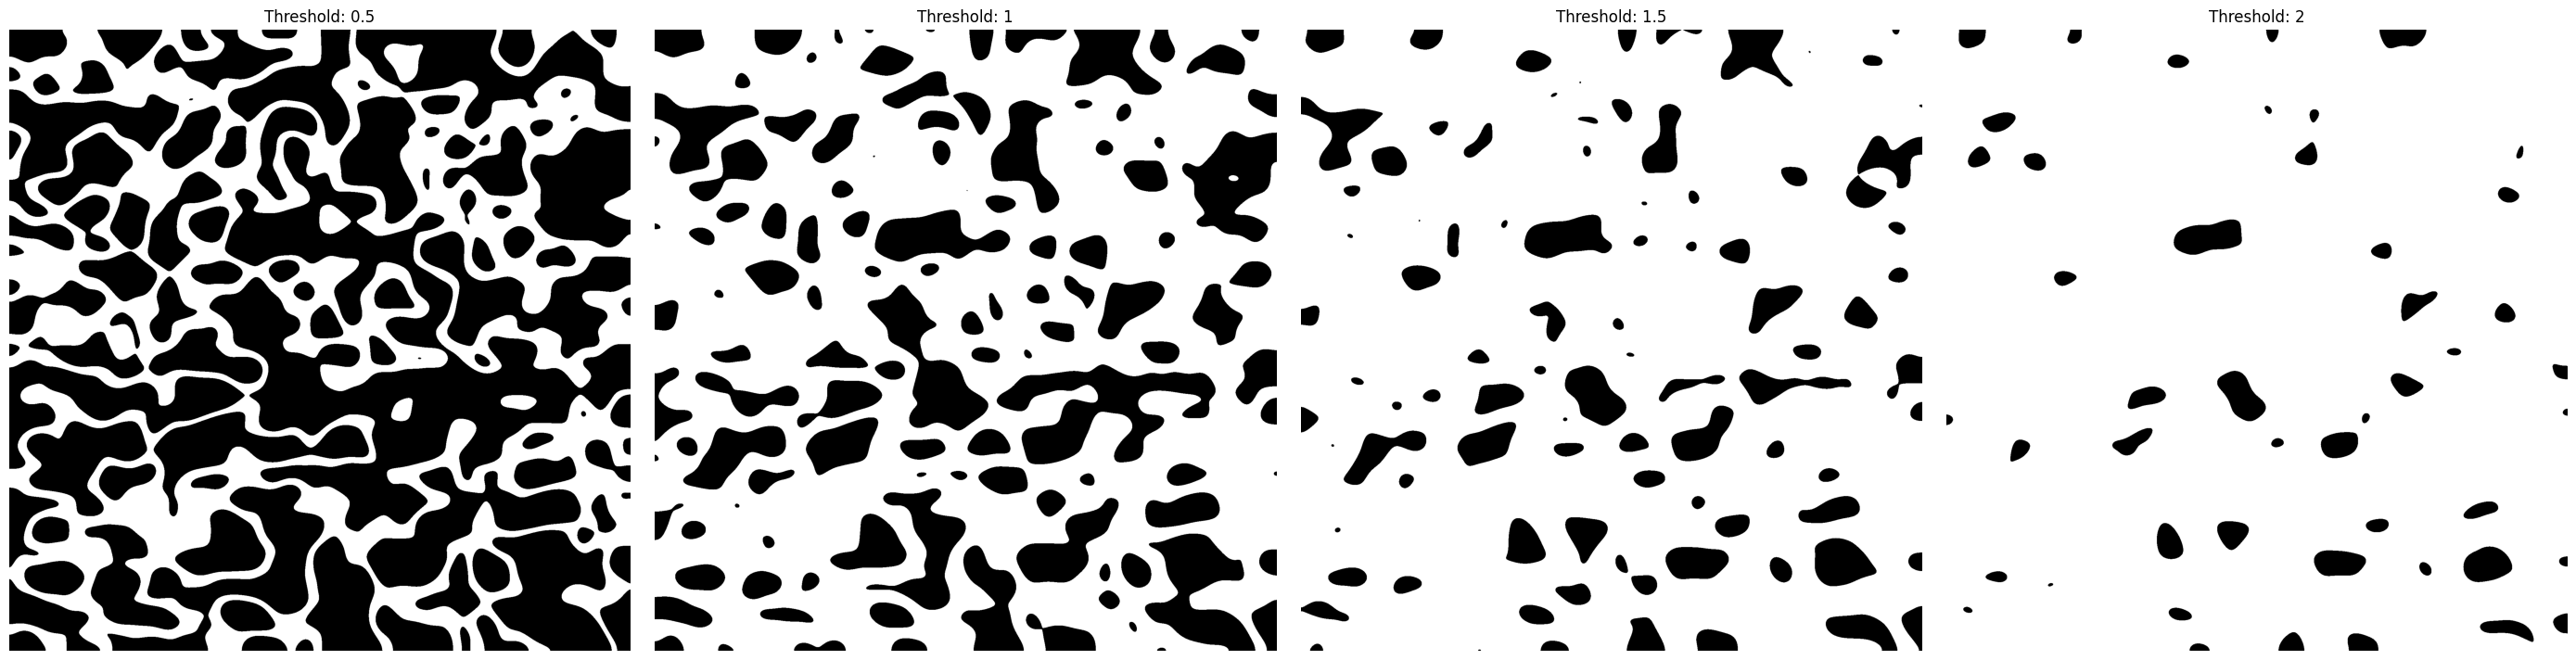
\includegraphics[width=\textwidth]{figures/threshold_comparison.png}
    \caption{Excursion sets $\Sigma(\nu) = \{ \kappa > \nu \sigma_0 \}$ for increasing thresholds ($\nu = 0.5, 1, 1.5, 2$). Black regions indicate areas where $\kappa$ exceeds $\nu \sigma_0$, showing reduced size and connectivity as $\nu$ increases.}
    \label{fig:excursion_sets}
\end{figure}

The Minkowski functionals $V_0(\nu_0)$, $V_1(\nu_0)$, and $V_2(\nu_0)$ quantify the morphological properties of these excursion sets \citep{2010PhRvD..81h3505M}: 
\begin{align}
    V_0(\nu_0) &= \frac{1}{A} \int_{\Sigma(\nu_0)} da, \label{eq:minkowski_V0} \\
    V_1(\nu_0) &= \frac{1}{4A} \int_{\partial \Sigma(\nu_0)} dl, \label{eq:minkowski_V1} \\
    V_2(\nu_0) &= \frac{1}{2\pi A} \int_{\partial \Sigma(\nu_0)} \mathcal{K} \, dl, \label{eq:minkowski_V2}
\end{align}
where $A$ is the total area, $da$ and $dl$ are area and length elements, and $\mathcal{K}$ is the geodesic curvature of the boundary $\partial \Sigma(\nu)$. Specifically: $V_0(\nu)$ measures the area fraction of the excursion set, $V_1(\nu)$ measures half the boundary length per unit area, and $V_2(\nu)$ quantifies the Euler characteristic per unit area.

For a pixelized map with $\nu_{\mathrm{pix}}$ pixels, the continuous integrals in Equations~\eqref{eq:minkowski_V0}--\eqref{eq:minkowski_V2} are approximated by discrete sums \citep{2012PhRvD..85j3513K}:
\begin{align}
    V_0(\nu_0) &\approx \frac{1}{N_{\mathrm{pix}}} \sum_{i=1}^{N_{\mathrm{pix}}} \Theta(\nu_i - \nu_0), \label{eq:V0_discrete} \\
    V_1(\nu_0) &\approx \frac{1}{4N_{\mathrm{pix}}} \sum_{i=1}^{N_{\mathrm{pix}}} \sum_{j \in \mathcal{N}(i)} |\Theta(\nu_i - \nu_0) - \Theta(\nu_j - \nu_0)|, \label{eq:V1_discrete} \\
    V_2(\nu_0) &\approx \frac{1}{2\pi N_{\mathrm{pix}}} \sum_{i=1}^{N_{\mathrm{pix}}} \delta_D(\nu_i - \nu_0) \left( \frac{\nu_{,xx} \nu_{,yy} - \nu_{,xy}^2}{\nu_{,x}^2 + \nu_{,y}^2} \right), \label{eq:V2_discrete}
\end{align}
where $\Theta$ is the Heaviside function, $\delta_D$ the Dirac delta function, $\mathcal{N}(i)$ the neighboring pixels of $i$, and derivatives are estimated via finite differences.

For a two-dimensional GRF $\kappa(\hat{\mathbf{n}})$ with zero mean and unit variance (after normalization), the Minkowski functionals are \citep{2010PhRvD..81h3505M}: 
\begin{align}
    V_0(\nu) &= \frac{1}{2} \operatorname{erf}\left( \frac{\nu}{\sqrt{2}} \right), \label{eq:V0_GRF} \\
    V_1(\nu) &= \frac{\sigma_1}{8\sqrt{2}\sigma_0} e^{-\nu^2/2}, \label{eq:V1_GRF} \\
    V_2(\nu) &= \frac{\sigma_1^2}{2\pi \sigma_0^3} \nu e^{-\nu^2/2}, \label{eq:V2_GRF}
\end{align}
where $\operatorname{erf}$ is the error function, and $\sigma_1^2 = \langle |\nabla \nu|^2 \rangle = \langle \kappa_{,x}^2 + \kappa_{,y}^2 \rangle$. These expressions provide a Gaussian benchmark for identifying non-Gaussian features in the data.